\documentclass[12pt]{article}
\usepackage{enumerate}
\usepackage{notes}
\usepackage{oxford}

\DeclareMathOperator{\diam}{\mathrm{diam}}


\begin{document}

\title{Oxford A2 - Metric Spaces and Complex Analysis
  \footnotetext{\url{https://courses.maths.ox.ac.uk/node/5378}}} \author{Dan Davison}
\maketitle

\section{Sheet 1}

\subsection{}
\begin{mdframed}
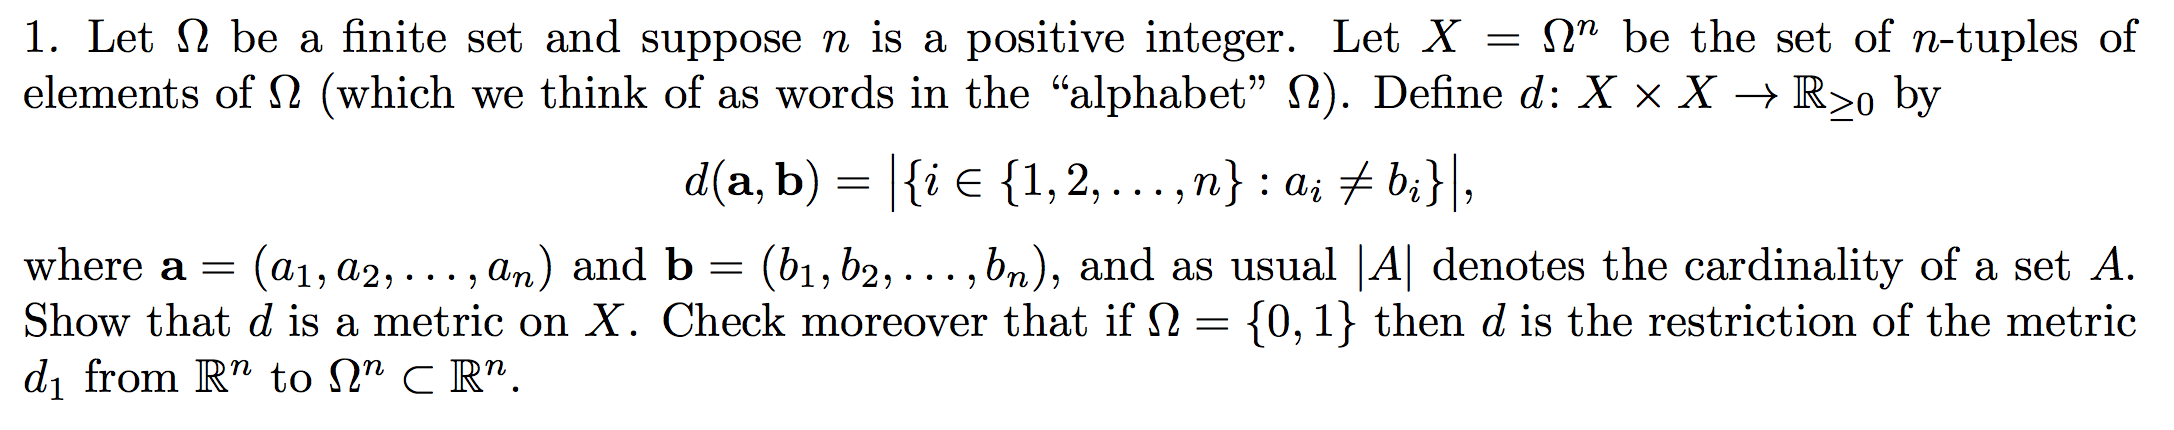
\includegraphics[width=400pt]{img/oxford-a2-1-1.png}
\end{mdframed}

\begin{remark*}
  $d$ is the Hamming distance.
\end{remark*}

For $d$ to be a metric on $X$ we require
\begin{enumerate}
\item \textbf{$d$ is a function $d:X \times X \to $ (a set of non-negative numbers).}\\
  Yes, this is true.
\item \textbf{Positivity}:\\
  Yes, cardinality is never negative and it is clear that $d(a,b) = 0 \iff a = b$.
\item \textbf{Symmetry}:\\
  Yes, follows from the fact that $a_i \neq b_i \iff b_i \neq a_i$.
\item \textbf{Triangle inequality}:\\
  % Want: $d(a, b) \leq d(a, c) + d(c, b)$ for all $a, b, c \in X$.
  Note that $d(a, b) = \sum_{i=1}^n \epsilon_{a_i,b_i}$, where $\epsilon_{ij} :=
  \begin{cases}
    0, ~~~ i = j\\
    1, ~~~ i \neq j
  \end{cases}
$ (the ``negation'' of the Kronecker delta).

  Fix $i \in \{1, 2, \ldots, n\}$. Suppose that $\epsilon_{a_i,b_i} = 0$. Then
  $\epsilon_{a_i,b_i} \leq \epsilon_{a_i,c_i} + \epsilon_{c_i,b_i}$. Alternatively suppose that
  $\epsilon_{a_i,b_i} = 1$. Then we have either $\epsilon_{a_i,c_i} = 0$, in which case
  $\epsilon_{c_i,b_i} = \epsilon_{a_i,b_i} = 1$, or we have $\epsilon_{a_i,c_i} = 1$.

  Therefore $\epsilon_{a_i,b_i} \leq \epsilon_{a_i,c_i} + \epsilon_{c_i,b_i}$, and therefore
  $\sumin \epsilon_{a_i,b_i} \leq \sumin \epsilon_{a_i,c_i} + \sumin \epsilon_{c_i,b_i}$, as required.
\end{enumerate}

Recall that $d_1:\R^n\times\R^n\to\R_{\geq 0}$ is given by $d_1(a, b) := \sum_{i=1}^n|a_i - b_i|$.

Let $\Omega = \{0, 1\} \subseteq \R$ and let $a, b \in \Omega^n \subseteq \R^n$.

Note that $|a_i - b_i| = \epsilon_{a_ib_i}$.

Therefore $d_1(a, b) = \sum_{i=1}^n\epsilon_{a_ib_i} = d(a, b)$, as required.

\newpage
\subsection{}
\begin{mdframed}
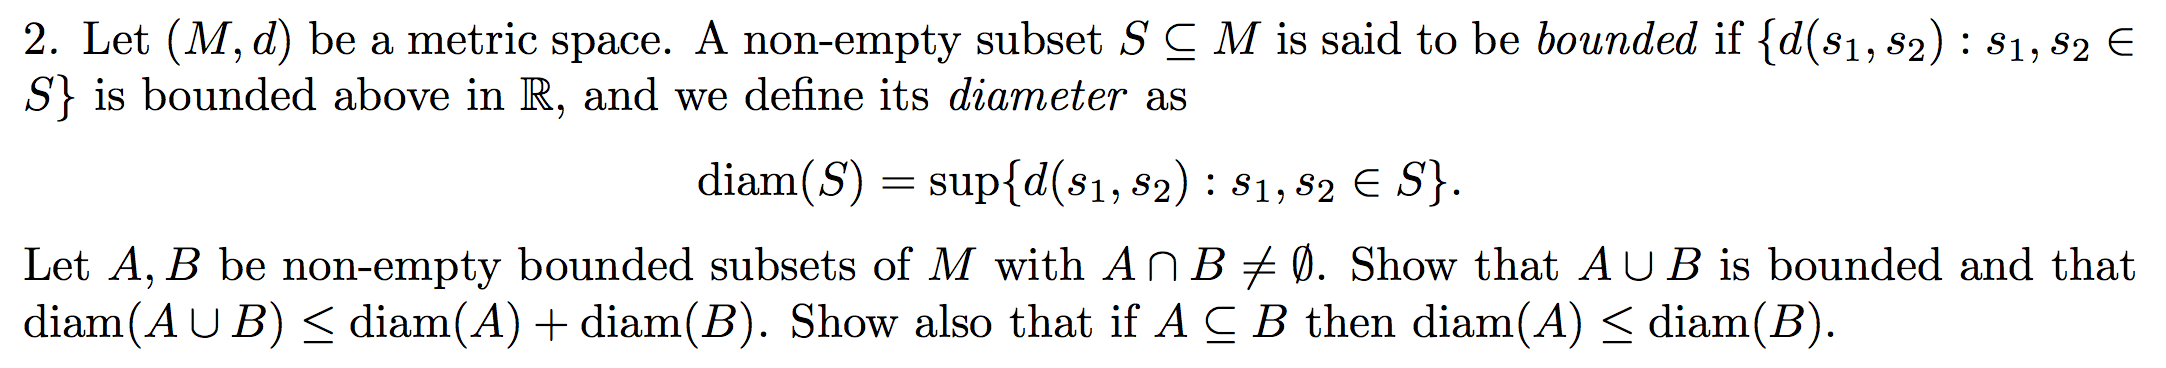
\includegraphics[width=400pt]{img/oxford-a2-1-2.png}
\end{mdframed}

\begin{claim*}
  $A \cup B$ is bounded and $\diam(A \cup B) \leq \diam(A) + \diam(B)$.
\end{claim*}

\begin{proof}
  Let $c_1, c_2 \in A \cup B$.

  Note that $c_1, c_2 \in A \implies d(c_1, c_2) \leq \diam(A)$ and
  $c_1, c_2 \in B \implies d(c_1, c_2) \leq \diam(B)$.

  Suppose, without loss of generality, that $c_1 \in A$ and $c_2 \in B$. Let $c_3 \in A \cap
  B$. Then by the triangle inequality we have
  $d(c_1, c_2) \leq d(c_1, c_3) + d(c_3, c_2) \leq \diam(A) + \diam(B)$.

  Therefore $A \cup B$ is bounded and $\diam(A \cup B) \leq \diam(A) + \diam(B)$.
\end{proof}


\begin{claim*}
  If $A \subseteq B$ then $\diam(A) \leq \diam(B)$.
\end{claim*}

\begin{proof}
  Let $A \subseteq B$, and suppose for a contradiction that $\diam(A) > \diam(B)$. Then there exist
  $a_1, a_2 \in A$ such that $d(a_1, a_2) > \diam(B)$. But since $A \subseteq B$ we have
  $a_1, a_2 \in B$. This contradicts the definition of $\diam(B)$ as the supremum over distances
  between pairs of elements of $B$. Therefore $\diam(A) \leq \diam(B)$.
\end{proof}


\newpage
\subsection{}
\begin{mdframed}
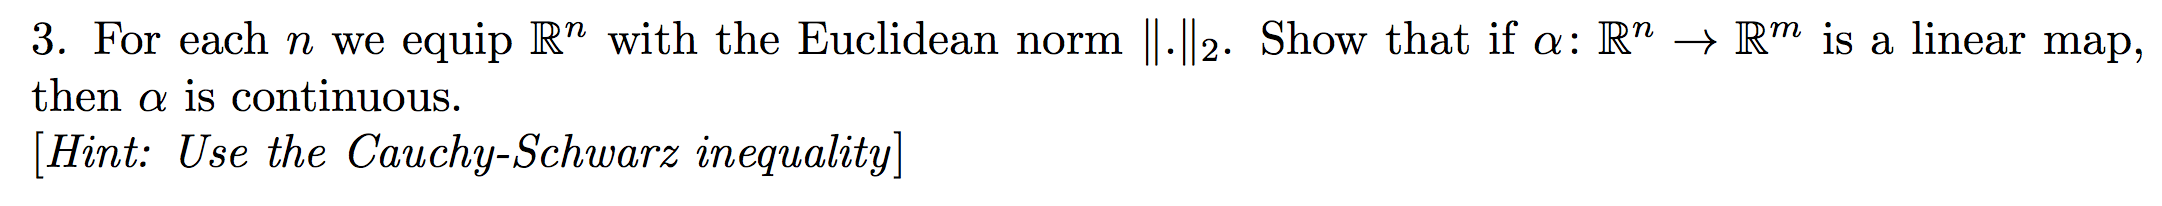
\includegraphics[width=400pt]{img/oxford-a2-1-3.png}
\end{mdframed}
\end{document}
